\documentclass{article}

%\usepackage[draft]{todonotes}
\usepackage{xcolor}
\usepackage[utf8]{inputenc}
\usepackage{mathtools}
\usepackage[utf8]{inputenc}
\usepackage[T1]{fontenc}
\usepackage[english]{babel}
\usepackage{graphicx}
%\usepackage{caption}
\usepackage{subcaption}
\usepackage{fixltx2e}
\usepackage{float}
\usepackage{amsthm}
\usepackage{amssymb}
\usepackage{booktabs}
\usepackage{enumitem} 
\newtheorem{definition}{Definition}
\newtheorem{theorem}{Theorem}
\usepackage{placeins}
\usepackage[a4paper, total={6in, 10in}]{geometry}


\numberwithin{equation}{subsection}
\setlength\parindent{0pt}
\setcounter{tocdepth}{2}


\begin{document}
	\section{Phylogenetic distance for constant populations}
	
	The purpose of this short manuscript is to see what information the phylogenetic distance distribution holds, and whether it might aid us in finding out the true $N$ or $p$ especially. The phylogenetic distance distribution is derived by first constructing a phylogenetic tree, and then you record the "distance" in terms of number of mutations on all edges in the tree.\\
	\\
	In figure \ref{fig::PDist}, you can see distributions of the phylogenetic distance for various values of p, with the $\mu$ changed to keep the $\mu_{eff}$ the same. The shape of the distribution looks roughly geometric and it is rather straightforward to show why it should be based on a small population of 3 individuals (though I can't show it yet for bigger populations). More importantly but unfortunately, the distribution stays exactly the same, so we can't find out anything about the p value this way. If we only vary the p or the $\mu$, they also simpley seem to change the distribution as predicted by the $ \mu_{eff}$. Which means that this distribution tells us exactly as much about the $p$ as the VAF does. \\
	\\
	Figure \ref{fig::TDist} also shows several distributions, now for varying values of t. Again, the distributions look extremely similar. In terms of mean distance, the lower times have a slightly lower value, but it rapidly approaches an asymptotic value. So, apart from a short time the population needs to approach an equilibrium in terms of distance, the t seems to have no influence on the distributions.\\
	\\
	Now a bit more interesting is the mean distance after a bottleneck event, varying N. This can be seen in figure  \ref{fig::NbnDistmean}. Evidently, there seems to be a simple linear relationship between N and mean distance with a slope of 1. This is unfortunately the same relationship as for the VAF-distribution.\\
	\\
	Lastly, we can look at the mean distance without a bottleneck (though this is arguably a bit more academic/impractical then with one, since this means we don't sample but look at the entire population anyway). As it is shown in figure \ref{fig::NDistmean}, there seems to be a logarithmic relationship between population size and mean distance when looking at the entire population.\\
	\\
	To conclude, the only difference between the distance and the VAF seems to be in a statistic not approachable for us, which is the mean distance for the entire population. Once we sample down, the distance distribution seems to lose information as to be effectively identical to the VAF in informational content.
	
	\begin{figure}[h!]
		\centering
		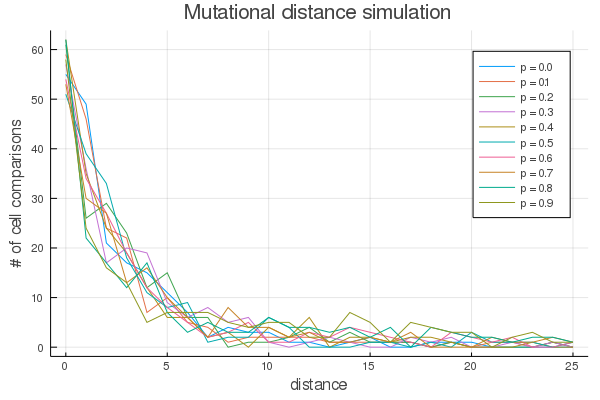
\includegraphics[width=\linewidth]{distance_N100_mu1.png}
		
		\caption{This figure shows the distribution of distances with varying p \& $\mu$ in such a way to keep the effective $ \mu_{eff} $ the same. On the x-Axis, we have the possible distances and on the y-Axis, the number of cell comparisons that have the respective distance. Parameters: $ N = 100$, $\mu_{eff} = 1 $, $ t = 100$.}
		\label{fig::PDist}
	\end{figure}
	
	\begin{figure}[h!]
		\centering
		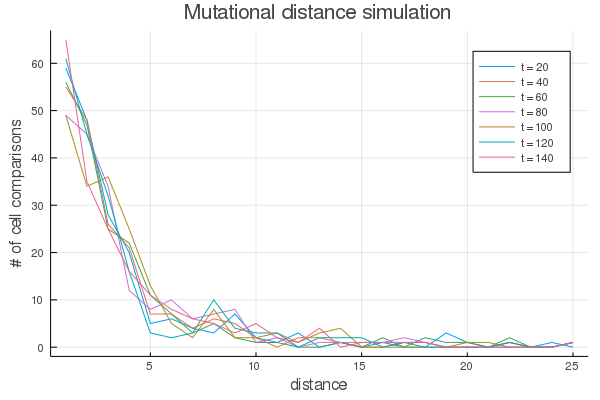
\includegraphics[width=\linewidth]{phyldistanceAll_N100.png}
		
		\caption{This figure shows the distribution of distances with varying t. On the x-Axis, we have the possible distances and on the y-Axis, the number of cell comparisons that have the respective distance. Parameters: $ N = 100$, $\mu_{eff} = 1 $.}
		\label{fig::TDist}
	\end{figure}

	\begin{figure}[h!]
		\centering
		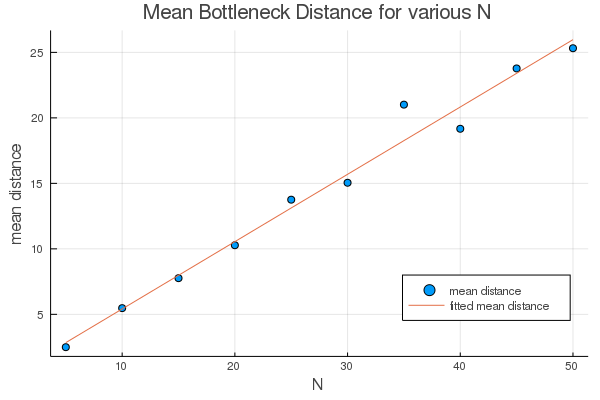
\includegraphics[width=\linewidth]{phyldistvarNbn_t200.png}
		
		\caption{This figure shows the mean distance with varying N after a bottleneck down to size 5. On the x-Axis, we have N and on the y-Axis, the corresponding mean distance. The fitted line is linear. Parameters: $ t = 200$, $\mu_{eff} = 1 $.}
		\label{fig::NbnDistmean}
	\end{figure}

	\begin{figure}[h!]
	\centering
	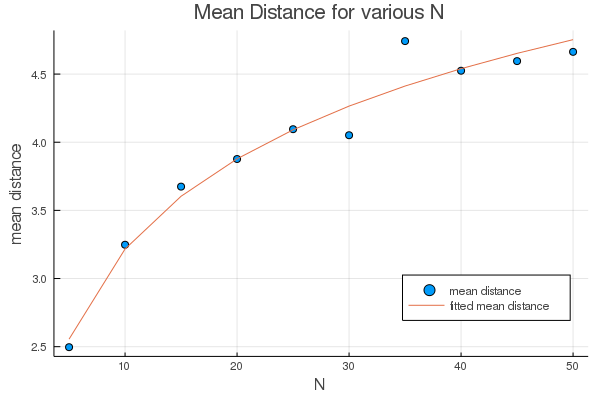
\includegraphics[width=\linewidth]{phyldistvarN_t200.png}
	
	\caption{This figure shows the mean distance with varying N without a bottleneck. On the x-Axis, we have N and on the y-Axis, the corresponding mean distance. The fitted line is logarithmic. Parameters: $ t = 200$, $\mu_{eff} = 1 $.}
	\label{fig::NDistmean}
\end{figure}

\end{document}